\documentclass{beamer}
\usepackage{graphicx}
\usepackage{amsmath}
\usepackage{amssymb}
\usepackage{tikz}
\usepackage{ctex}
\usepackage{multicol}
\usepackage{hyperref}
\usepackage{ifthen}

\usetheme{Berlin}
\usefonttheme{serif}
\setbeamercovered{dynamic}

\graphicspath{{./image/}}

\usepackage{etoolbox}
\AtBeginSection{
  \frame{\sectionpage}
  \begin{frame}{本节内容}

      \begin{columns}[T]
        \column{0.48\textwidth}
        \tableofcontents[sections={1-\the\numexpr\value{section}/2\relax},currentsection]
        
        \column{0.48\textwidth}
        \tableofcontents[sections={\the\numexpr\value{section}/2+1\relax-},currentsection]
      \end{columns}

  \end{frame}
}

\AtBeginSubsection{
    \frame{\subsectionpage}
}

\title{LCPU 先导课:计算机基础}
\author{臧炫懿}
\institute{北京大学 信息科学技术学院}
\date{\today}

\begin{document}

\frame{\titlepage}

\section{计算机基础知识}

\subsection{计算机的历史}
\begin{frame}{计算机的鼻祖}
    \begin{columns}[T]
        \column{0.48\textwidth}
            \begin{itemize}
                \item <1->图灵机
                \item <2->冯·诺依曼架构
            \end{itemize}

        \column{0.48\textwidth}
            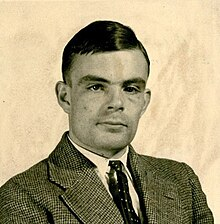
\includegraphics[width=0.9\textwidth]{1-1-Turing.jpg}
    \end{columns}
\end{frame}

\subsection{计算机的组成}

\begin{frame}{计算机的硬件}
    \begin{columns}[T]
        \column{0.48\textwidth}
            计算机的\textbf{硬件},也可以叫做\textbf{设备},可以简单分为两类:一类叫做\textbf{主机设备},是计算机用来进行计算等工作的设备;另一类叫做\textbf{外设设备}(也可以叫做\textbf{输入输出设备}),是计算机与外界进行信息交互的设备。通常说来,前者是藏在机箱里看不见的,后者是我们能够直接看见的。

            一个计算机的主机设备如右图。
        
        \column{0.48\textwidth}
            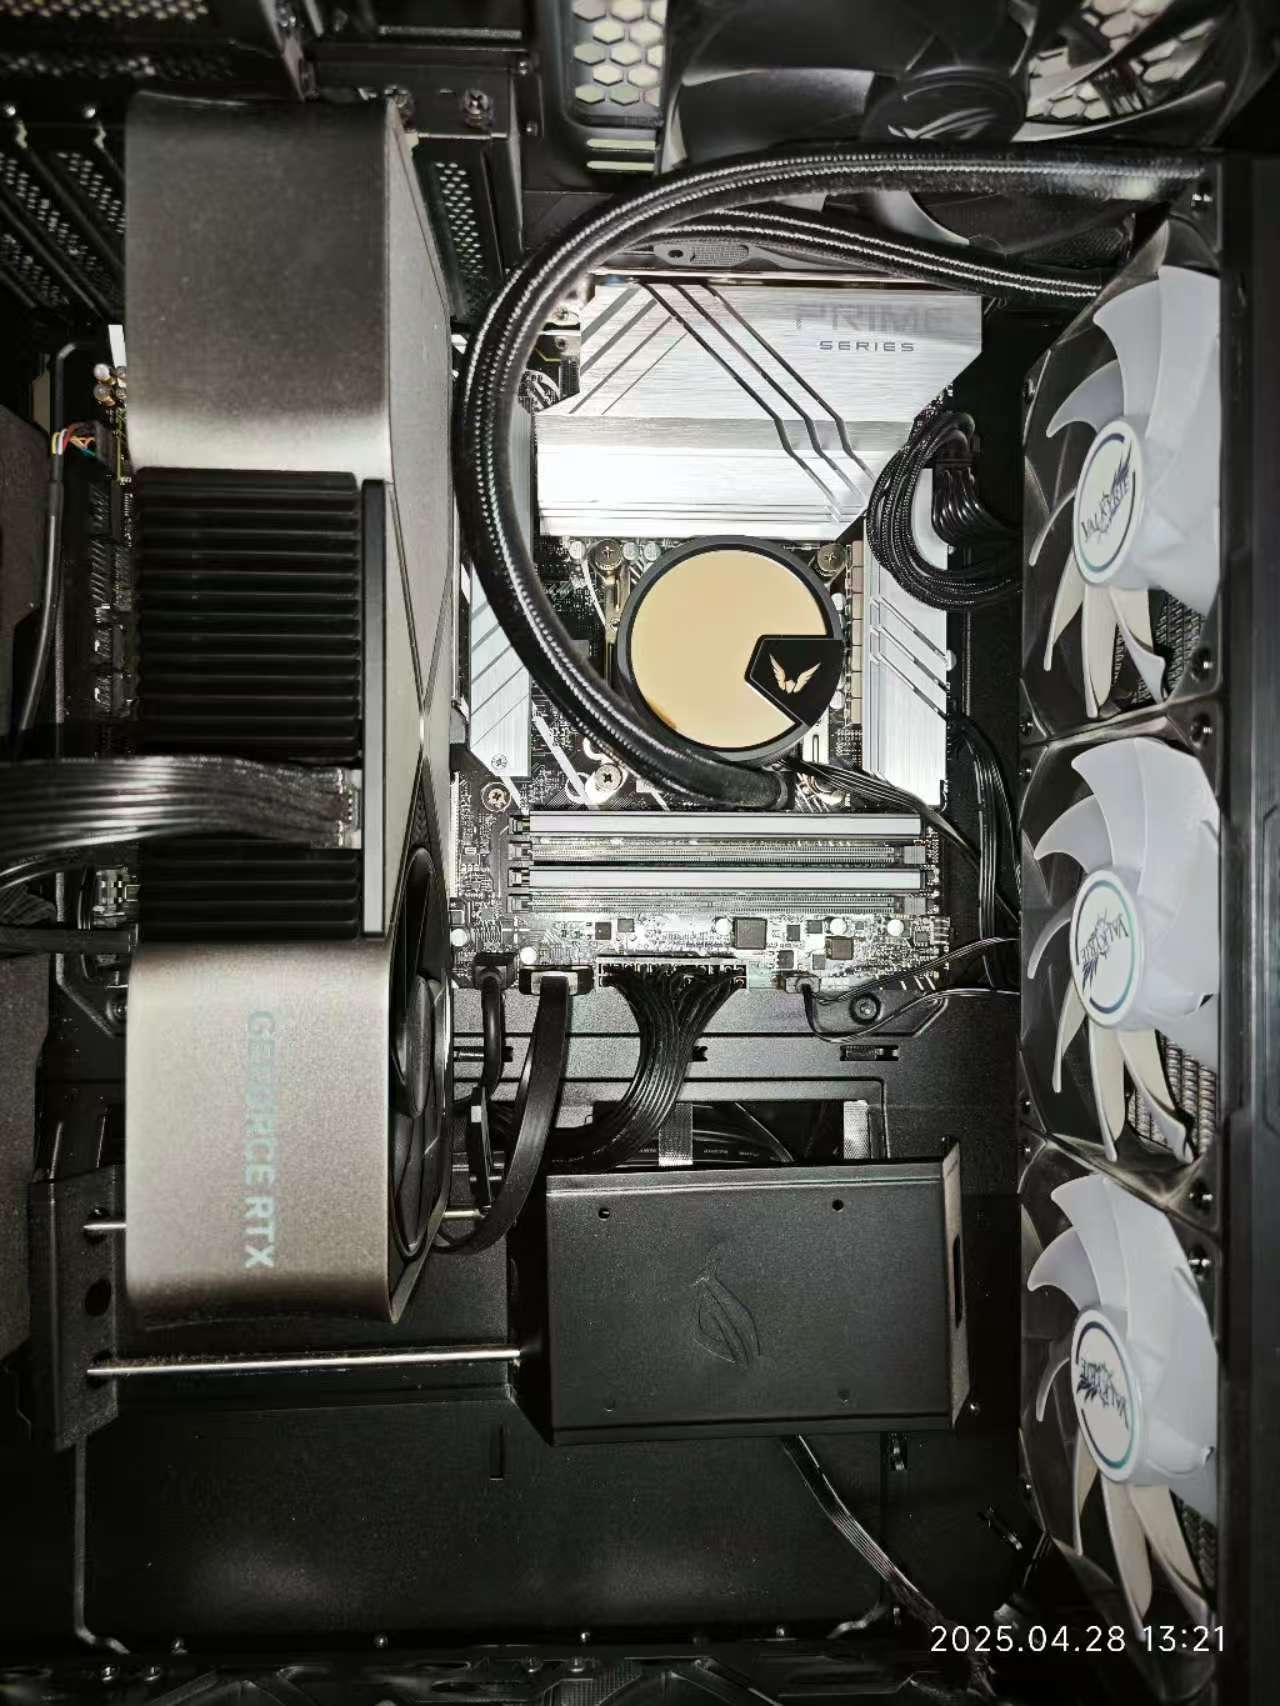
\includegraphics[width=0.7\textwidth]{1-2-Hardware.jpg}
    \end{columns}
\end{frame}

\begin{frame}{中央处理器}
    \textbf{中央处理器}也被称为是\textbf{CPU},是计算机的最核心部件。它负责执行程序指令和进行算术逻辑运算。虽然现代处理器对代码和数据的处理不尽相同,但我们可以把它们都看作是\textbf{指令}。
    
    在运行程序时,CPU会按照顺顺序,一条一条执行从存储设备中读取的指令(至少从软件和程序员等使用者的视角看是这样),指令可以是修改CPU的状态、进行运算、从其他硬件读取信息或者输出信息等。
\end{frame}

\begin{frame}{内存}
    \textbf{内存}是计算机的临时存储器,它用于存储正在运行的程序和数据。它能够被CPU直接访问,因此速度较快。对于程序员而言,内存可以被抽象为一堆连续的存储单元,每个存储单元都有一个唯一的地址;执行程序时,程序的一部分或者全部被放进内存中,CPU 就在内存中找寻需要的数据或者指令。

    内存在断电后数据会被清空,因此它通常被称为\textbf{易失性存储器}。又因为它可以在任意时刻访问任意地址,所以它也被称为\textbf{随机存取存储器}或者\textbf{RAM}。在其他语境下,内存有不同的含义,应该根据上下文加以区分。
\end{frame}

\begin{frame}{外存}
    \textbf{外存}是现代计算机的主要存储设备,用于存储操作系统、应用程序和数据等内容。其读写速度往往比内存慢得多,但是它的存储容量更大且往往是\textbf{非易失的}。

    现代计算机的主要外存设备是\textbf{硬盘}。硬盘可以分为机械硬盘(HDD)和固态硬盘(SSD)。机械硬盘使用磁头在旋转的磁盘上读取和写入数据,而固态硬盘使用闪存芯片来存储数据。固态硬盘的读写速度比机械硬盘快得多,现在价格也便宜得多,但是使用寿命较短,不适宜长期存储重要数据。
\end{frame}

\begin{frame}{其他外存设备}
    除了硬盘,计算机还有其他的常见外存设备。

    \begin{itemize}
        \item 光盘
        \item U盘
        \item 磁带
        \item 软盘
    \end{itemize}
\end{frame}

\begin{frame}{显卡}
    \textbf{显卡}是计算机的图形处理器,用于处理图像和视频等数据。它可以将计算机生成的图像转换为显示器可以理解的格式,并将其输出到显示器上。显卡通常有自己的内存,用于存储图像数据和纹理等信息。显卡的计算核心是\textbf{GPU},与CPU的一个重要区别在于,GPU的计算核心数量远多于CPU的计算核心数量,但是每个核心的计算能力较弱。

    对于AI时代来说,显卡因为其强大的并行计算能力,成为了深度学习等领域的主要计算设备。显卡的计算能力通常用\textbf{浮点运算能力}来衡量,单位是\textbf{FLOPS}(每秒浮点运算次数)。
\end{frame}

\begin{frame}{主板、电源}
    \textbf{主板}是一块电路板,将所有的硬件设备连接起来。主板上的芯片组负责协调各个硬件之间的通信。同时,主板还有一系列外部接口,用于连接外部设备。

    \textbf{电源}是计算机的电源供应器,它不参与数据存储与运算等操作,但能够为计算机的各个部件提供所需的稳定工作电压和电流。优质的电源能够避免计算机在运行过程中出现故障,延长计算机的寿命。
\end{frame}

\begin{frame}{输入输出设备}
    \textbf{输入设备}是计算机与外界进行信息交互的设备,用于将用户的输入转换为计算机可以理解的格式。最古老的输入设备是拔插电缆,后来变成打孔纸带;现代常见的输入设备包括键盘、鼠标、扫描仪、麦克风等。
    
    \textbf{输出设备}则相反,把计算机处理后的数据转换为用户可以理解的格式,例如显示器、打印机、音响等。
\end{frame}

\begin{frame}{软件}
    \textbf{软件}是计算机的程序和数据的集合。它可以分为系统软件和应用软件两大类。

    \begin{itemize}
        \item 系统软件:操作系统、驱动程序等
        \item 应用软件:办公软件、游戏、浏览器等
    \end{itemize}

    如果说硬件是计算机的身体,那么软件就是计算机的灵魂。没有软件,计算机就无法发挥作用;没有硬件,软件也无法运行。
\end{frame}

\begin{frame}{操作系统}
    \textbf{操作系统}是计算机的核心软件,负责管理计算机的硬件和软件资源。它提供了一个用户与计算机交互的界面,并为应用程序提供了一个运行环境。常见的个人PC操作系统有:

    \begin{itemize}
        \item Windows
        \item macOS
        \item Linux
    \end{itemize}
\end{frame}

\begin{frame}{操作系统的对比}
    \textbf{Windows}是微软公司开发的操作系统,占有目前最大的市场份额。它的优点是易于使用,兼容性好,支持大量的应用程序;缺点是安全性差,且不适宜进行一些较为专业的任务,例如高性能计算、软件开发、深度学习等。

    \textbf{macOS}是苹果公司开发的操作系统,主要用于苹果公司的计算机产品。它的优点是界面美观,易于使用,安全性较高;缺点是兼容性稍差,主要支持苹果公司的硬件产品,且价格较贵;而这些硬件产品往往也和其他操作系统间兼容性较差。

    \textbf{Linux}是一个开源的操作系统,广泛应用于服务器、嵌入式系统等领域,目前已经有多个发行版,例如Ubuntu、Debian、Arch等。它的优点是安全性高、稳定性好、性能强大;缺点是学习曲线陡峭,使用不够友好。
\end{frame}

\begin{frame}{驱动程序}
    \textbf{驱动程序}是操作系统和硬件之间的桥梁。它负责将操作系统的指令转换为硬件可以理解的格式,并将硬件的状态反馈给操作系统。每个硬件设备都需要一个对应的驱动程序才能正常工作。

    驱动程序通常由硬件制造商提供,用户在安装新硬件时需要利用附带光盘安装相应的驱动程序(如打印机)。我们也可以通过操作系统的更新来更新驱动程序,或者前往硬件制造商官网来获取驱动程序。但是,我们不推荐使用“驱动精灵”等第三方软件来更新驱动程序,因为它们可能会安装不必要的驱动程序,并导致系统不稳定。
\end{frame}

\begin{frame}{应用软件}
    \textbf{应用软件}则是计算机上运行的各种程序,一般用于实现某个或者某些特定的功能,例如QQ等即时通讯软件、Chrome等浏览器等。

    我们下载软件的主要渠道有两个:一个是通过官方渠道(如软件官网、Microsoft Store、学校和公司提供的其他方式)下载,另一个是通过包管理器(Winget、Homebrew、Apt、Pacman等)下载。我们不推荐在非官方渠道下载软件,因为它们可能会捆绑恶意软件,导致计算机感染病毒、木马等恶意程序。
\end{frame}

\begin{frame}{北京大学正版软件}
    为了保护知识产权、方便学生节约资金,北京大学购买了一系列常用软件的正版授权,方便师生使用。我们可以登录\href{https://software.pku.edu.cn/}{北京大学正版软件网站},使用自己的北大账号和密码登录,下载和安装这些软件。
\end{frame}

\section{网络及其配置}

% 这一段将会由其他人讲授!

\section{计算机进阶}

\subsection{维护你的系统}
\begin{frame}{按需更新系统和软件} 
    计算机在运行过程中,操作系统和软件会不断地更新,以修复漏洞、提高性能和增加新功能。我们应该定期检查系统和软件的更新,并及时按需要安装它们。

    对于一些重要的更新(例如安全更新等),我们应该立即安装,这是因为此类更新通常是为了修复一些新近发现的漏洞和问题,如果不及时安装,可能会导致计算机被攻击或者出现其他问题。而对于一些不重要的更新(例如功能更新等),我们可以根据自己的需要选择安装。
\end{frame}

\begin{frame}{定期备份数据}
    定期备份数据是保护计算机数据安全的重要措施。我们可以使用外部硬盘、云存储等方式备份数据,以防止信息泄露或者重要文件丢失。数据备份的频率可以根据数据的重要性和变化频率来决定。

    数据备份有一个重要的原则:\textbf{3-2-1备份法则}。即:至少保留三份数据备份,存储在两个不同的介质上,其中一份存储在异地。例如,我们可以在本地硬盘上存储一份数据备份,在外部硬盘上存储一份数据备份,并将另一份数据备份存储在云端。这样,即使其中一份甚至两份损坏或者丢失,我们也可以通过其他方式恢复数据。
\end{frame}

\begin{frame}{定期清理系统}
    定期清理系统可以提高计算机的性能和安全性。我们可以使用一些系统清理工具,删除不必要的文件、缓存和临时文件等,以释放磁盘空间和提高系统性能。我们推荐使用系统自带的清理工具,例如Windows的磁盘清理工具、macOS的存储管理工具等;也可以使用一些知名的清理软件,例如CCleaner等。出于众所周知的原因,不建议使用类似于360等清理软件。
\end{frame}

\begin{frame}{碎片整理}
    在计算机使用过程中,如果使用机械硬盘,文件的删除和修改会导致磁盘上的数据变得零散,从而影响计算机的性能。我们可以使用碎片整理工具,定期对磁盘进行碎片整理(即重排文件使其连续),以部分提高磁盘的读写速度。

    直接使用Windows自带的碎片整理工具即可。对于固态硬盘,碎片整理并不会提高性能,反而会缩短使用寿命,因此不建议对SSD进行碎片整理。
\end{frame}

\begin{frame}{放空C盘}
    对于Windows系统而言,C盘是最重要的磁盘或磁盘分区之一。它通常用于存储操作系统和应用程序等重要文件。

    任何时候,建议C盘的剩余空间都应该保持在20\%以上。否则,可能会导致系统运行缓慢。然而,C盘的重要性使我们一般不建议直接删除C盘中的文件。除了清理不必要的文件和缓存外,我们应该从源头解决问题,也就是尽可能地将文件存储在其他磁盘上,并将软件也存储在其余磁盘上。
\end{frame}
\subsection{善用终端和快捷键}

\begin{frame}{终端}
    \textbf{终端}是计算机与操作系统之间的一个交互界面。它允许用户通过命令行输入指令,与操作系统进行交互。

    虽然终端是一个非常古老的工具,但是使用它依然可以提高工作效率,尤其是在处理大量文件或者进行复杂操作时。它还可以用于远程连接到其他计算机,进行远程管理和维护等操作。

    对于Linux和macOS,我们建议使用Zsh或Fish等更加友好的shell,他们能够进行语法高亮、自动补全等操作。对于Windows,我们建议使用Windows Powershell。Powershell和Linux的shell的命令行上有很大的不同,这是因为Powershell的设计理念是模仿C\#的“对象”。不过也正因此,Powershell本身就是一门完备的语言,功能非常强大,能够处理相当复杂的任务。
    
\end{frame}

\begin{frame}{快捷键}
    使用快捷键可以减少鼠标操作的频率。以下是来自Windows的常用快捷键:
    \begin{columns}[T]
        \column{0.48\textwidth}
            \begin{itemize}
                \item Ctrl+C:复制
                \item Ctrl+V:粘贴
                \item Ctrl+Z:撤销
                \item Ctrl+Y:重做
                \item Ctrl+A:全选
                \item Ctrl+Alt+Del:任务管理器
                \item Alt+F4:关闭窗口
            \end{itemize}

        \column{0.48\textwidth}
            \begin{itemize}
                \item Win+R:打开运行窗口
                \item Win+E:文件资源管理器
                \item Win+D:显示桌面
                \item Win+L:锁定计算机
                \item Ctrl+S:保存
                \item Ctrl+P:打印
                \item Ctrl+F:查找替换
            \end{itemize}
    \end{columns}
\end{frame}
\subsection{版本控制}
\begin{frame}
    \frametitle{版本控制}
    \textbf{版本控制}是指对计算机文件的不同版本进行管理和跟踪的过程。它可以帮助我们记录文件的历史版本,方便我们在需要时恢复到之前的版本。

    目前最流行的版本控制系统是\textbf{Git}。Git是一个分布式版本控制系统,允许多个用户在不同的计算机上对同一个项目进行协作开发。它可以记录每次修改的历史记录,并允许用户随时回退到之前的版本。
\end{frame}

\begin{frame}
    \frametitle{Git的工作原理}
    Git的工作由三个目录共同完成:工作区、暂存区和版本库。

    \textbf{工作区}是我们实际操作的目录,包含了我们正在编辑的文件;\textbf{暂存区}是一个临时存储区域,用于暂时保存我们准备提交的文件;\textbf{版本库}用于存储所有的版本信息。版本信息是一个“节点”,包含了文件的快照、提交信息等。同时,还有一个指针,指向当前版本的最新提交。
\end{frame}

\begin{frame}
    \frametitle{Git的基本命令}
    \begin{itemize}
        \item git init:初始化一个新的Git仓库
        \item git add:将文件添加到暂存区
        \item git commit:提交暂存区的更改到本地仓库
        \item git restore:将文件从暂存区恢复到工作区
        \item git reset:将文件从版本库恢复到工作区
        \item git status:查看当前工作区和暂存区的状态
        \item git log:查看提交历史
    \end{itemize}
\end{frame}
\subsection{网络安全}

\begin{frame}{网络安全}
    虽然互联网的出现给我们带来了便利,但也带来了很多风险。部分人心术不正,使
    用互联网进行诈骗、盗窃、敲诈勒索等违法犯罪活动;而他们使用的主要手段是不定向的网络攻击,例如钓鱼、木马、蠕虫和病毒等。
\end{frame}

\begin{frame}{从根源解决问题}
    为了防止计算机被感染或者破坏,我们应该从源头解决问题。我们可以采取以下措施:
    \begin{itemize}
        \item <2->不浏览不安全网页或下载不明软件;
        \item <3->识别伪造的网站;
        \item <4->保持操作系统和软件的更新;
        \item <5->使用防火墙和杀毒软件;
        \item <6->使用强密码和密钥等更加安全的措施;
        \item <7->善用沙箱;
        \item <8->定期备份数据并创建系统还原点。
    \end{itemize}
\end{frame}

\begin{frame}{亡羊补牢的办法}
    如果不幸感染了病毒或者木马,我们可以采取以下措施:
    \begin{itemize}
        \item <2->立刻断开网络连接;
        \item <3->使用杀毒软件进行全面扫描;
        \item <4->向有关部门报告;
        \item <5->使用系统还原点恢复或重装操作系统。
    \end{itemize}
\end{frame}

\section{搜索和信息获取}

\subsection{信息的鉴别}
\begin{frame}
    \frametitle{信息的鉴别}
    在互联网时代,信息的获取变得非常容易,但是信息的质量却参差不齐。我们在了解如何获取信息前,应该学会鉴别信息的真实性和可靠性。

    一般我们可以从以下几个方面来判断信息的真实性和可靠性:
    \begin{itemize}
        \item <2->来源:是否来自权威机构或专业人士?
        \item <3->内容:是否有事实依据和数据支持?
        \item <4->时间:是否是最新的?是否已经过时?
        \item <5->可验证性:是否可以通过其他渠道验证?
        \item <6->评价:其他人对该信息的评价如何?认可度高吗?
    \end{itemize}
\end{frame}

\subsection{搜索及其技巧}

\begin{frame}{选择搜索引擎}
    \begin{columns}[T]
        \column{0.48\textwidth}
            国内最常用的搜索引擎是百度。但是我们在使用百度搜索的时候,往往会遇到一些问题,例如搜索结果不准确、广告太多等。其他国内搜索引擎也有类似的问题,因此并不好用。
        \column{0.48\textwidth}
            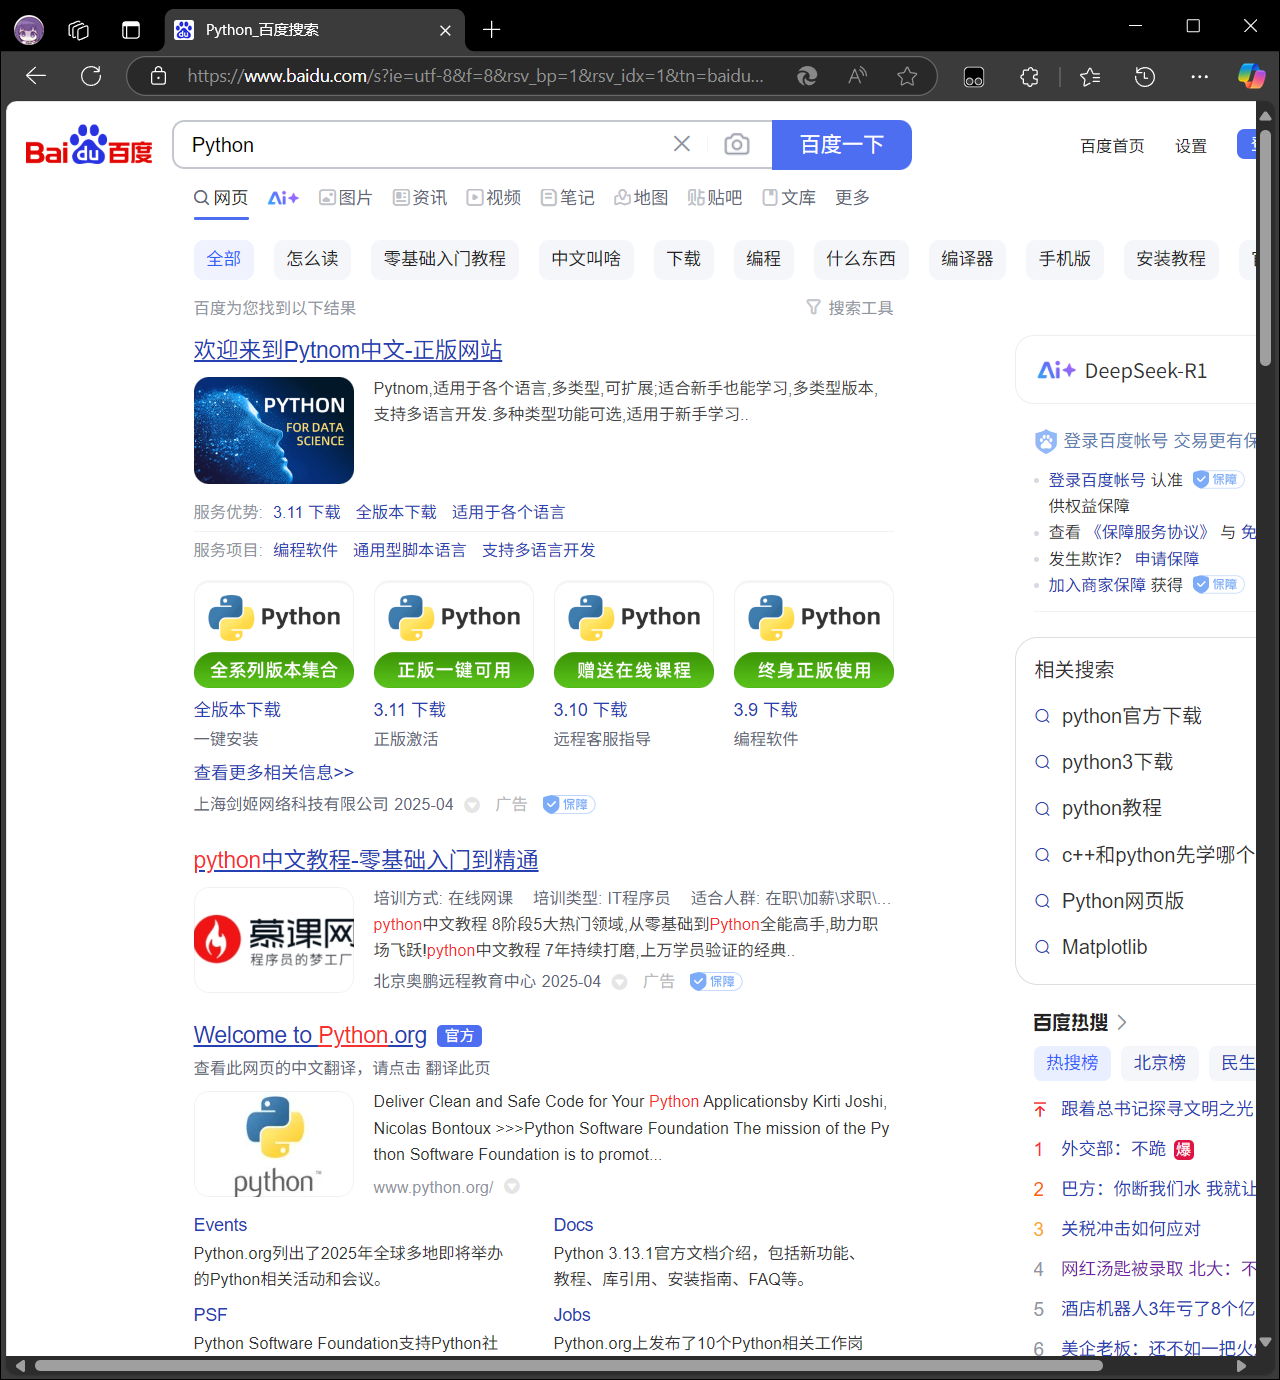
\includegraphics[width=0.9\textwidth]{4-1-Baidu.png}
    \end{columns}
\end{frame}

\begin{frame}{选择搜索引擎}
    \begin{columns}[T]
        \column{0.48\textwidth}
            目前新购整机几乎都已经预装了Windows 11,Windows 11自带的搜索引擎是必应(Bing)。我们可以在Bing的界面顶端发现两个按钮,分别是“国内版”和“国际版”。其中,国内版的搜索结果也不尽如人意。
        \column{0.48\textwidth}
            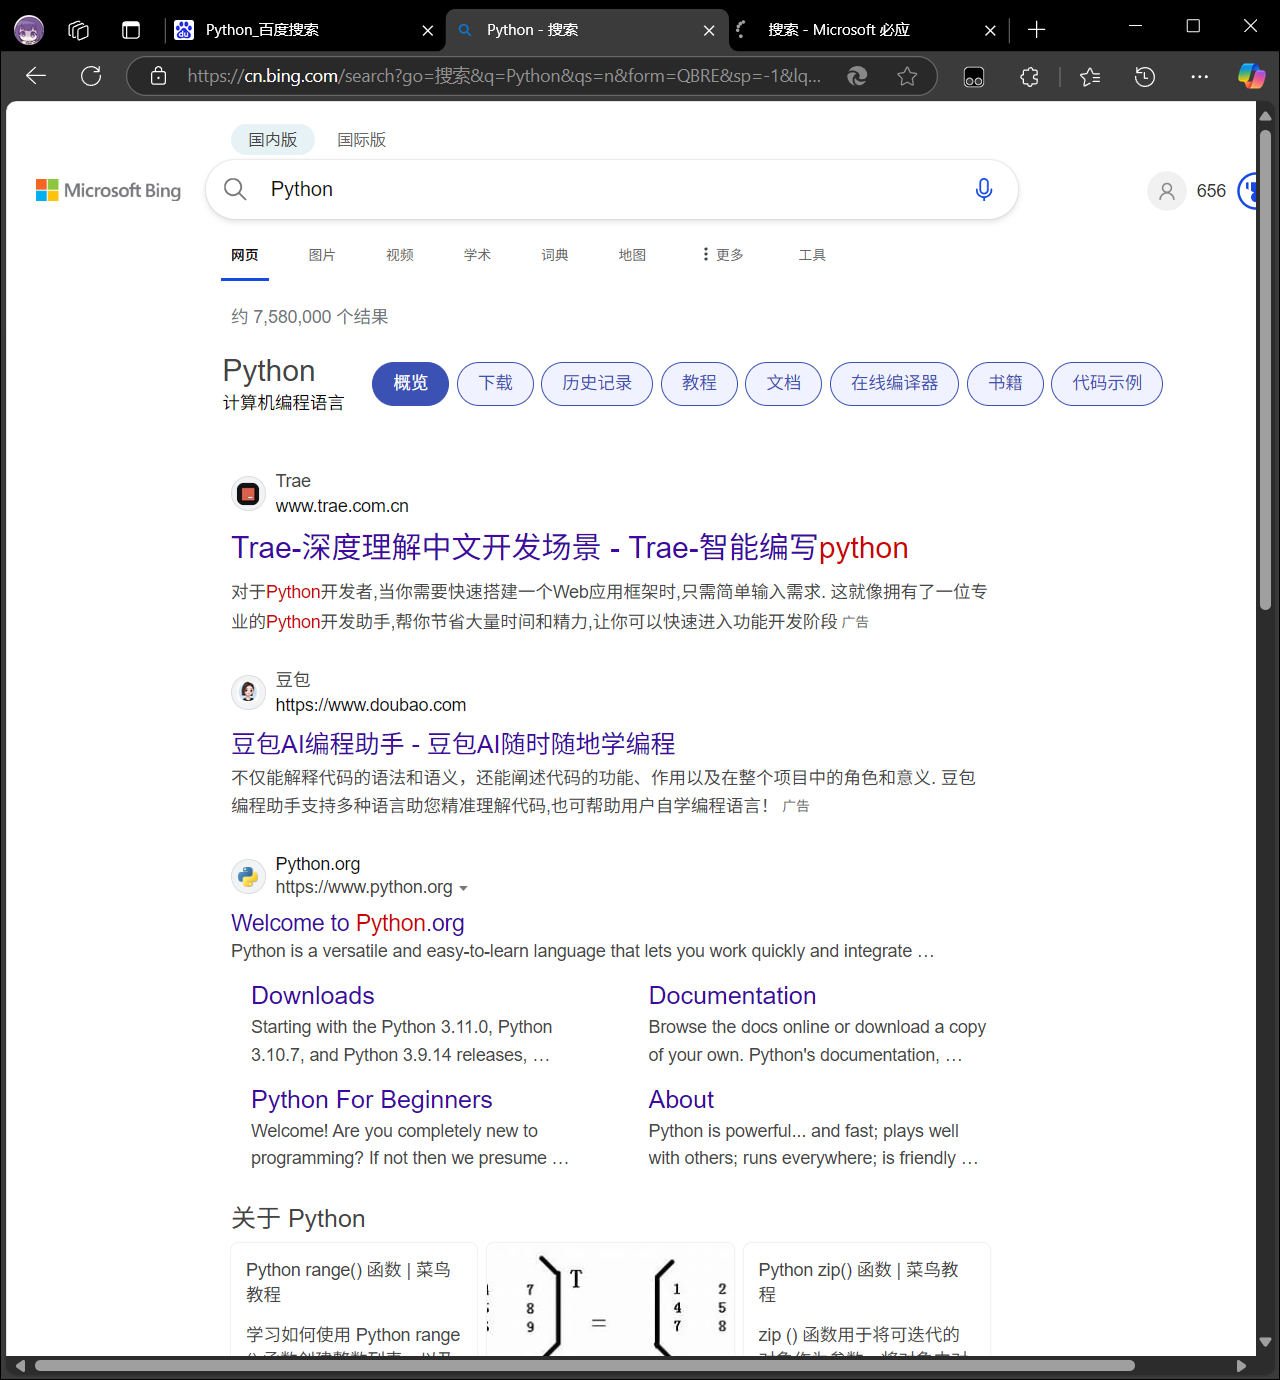
\includegraphics[width=0.9\textwidth]{4-2-BingN.png}
    \end{columns}
\end{frame}

\begin{frame}{选择搜索引擎}
    \begin{columns}[T]
        \column{0.48\textwidth}
            而如果使用国际版的Bing搜索引擎,我们会发现它的搜索结果非常准确,且广告也很少。因此,我们建议,如果需要搜索的内容\textbf{非中文社区独有},则可以使用国际版的Bing搜索引擎。另一个更好的选择是Google,但是可惜的是在国内一般无法访问。
        \column{0.48\textwidth}
            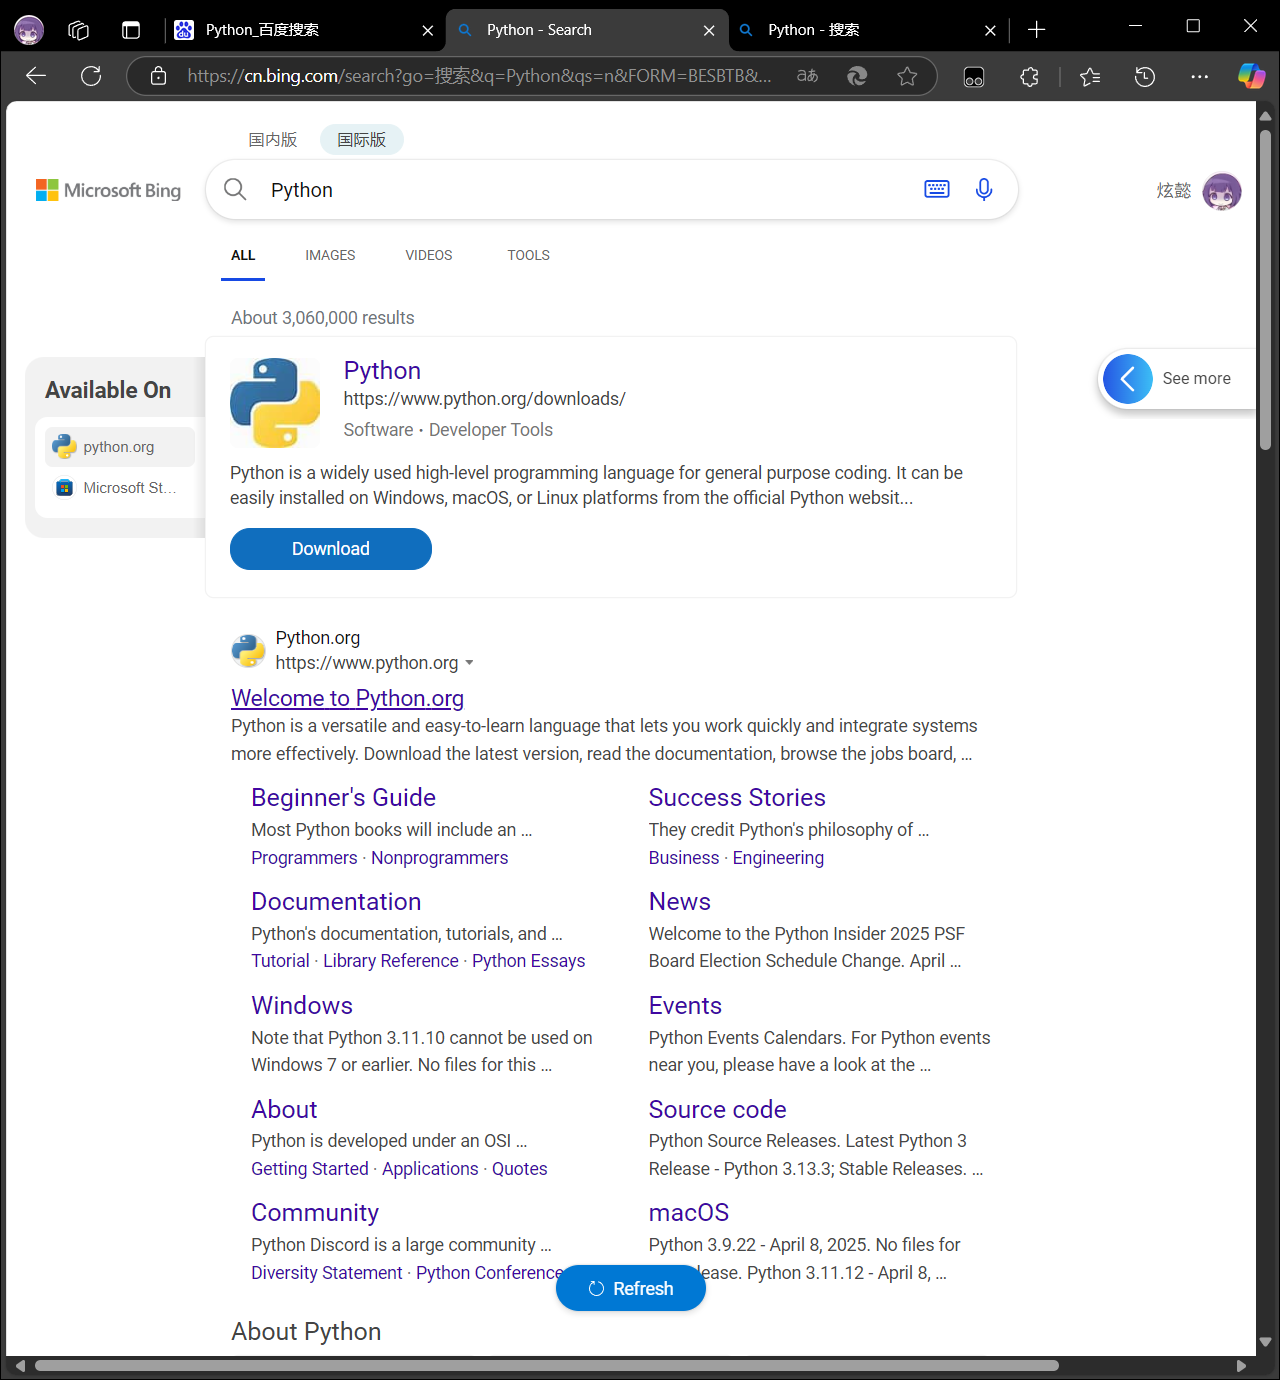
\includegraphics[width=0.9\textwidth]{4-3-BingI.png}
    \end{columns}
\end{frame}

\begin{frame}{搜索的技巧}
    有时候我们搜索的时候无法找到我们想要的结果,这时候我们可以使用一些搜索技巧来提高搜索的效率。

    \begin{itemize}
        \item <2->使用关键词搜索;
        \item <3->使用英语;
        \item <4->使用高级搜索选项;
        \begin{itemize}
            \item <5->引号、减号、星号;
            \item <6->site:、filetype:
        \end{itemize} 
    \end{itemize}
\end{frame}

\subsection{信息平台的选取}

\begin{frame}{官方文档、Wiki、论坛}
    如果我们希望获取某个软件的信息,最好的地方往往是它的官方文档。官方文档通常是最权威、最准确的信息来源,包含了软件的安装、使用和配置等信息。
    
    对于Arch Linux这类完全由社区维护的项目,其Wiki和论坛也是获取信息的最佳选择之一。虽然上述文档等可能存在晦涩难懂的地方,但是它们通常是最准确的信息来源。
    \begin{block}{小提示}<2->
        如果你在提问时遇到了诸如RTFM(Read The F***ing Manual)等回复,说明答主认为你应认真阅读官方文档。当然,这种情况下\textbf{他大概率是对的,你应该去读一读。}而通过自行查找而不是直接告诉你答案,你也能学到更多东西。
    \end{block}
    
\end{frame}

\begin{frame}{堆栈溢出}
    \begin{columns}[T]
    \column{0.48\textwidth}
        堆栈溢出(Stack Overflow)是一个程序员问答网站,用户可以在上面提问和回答问题。它的内容主要是关于编程、计算机科学和软件开发等方面的问题。

        从我个人的使用体验而言,这东西有点像百度贴吧和知乎的结合体。

    \column{0.48\textwidth}
        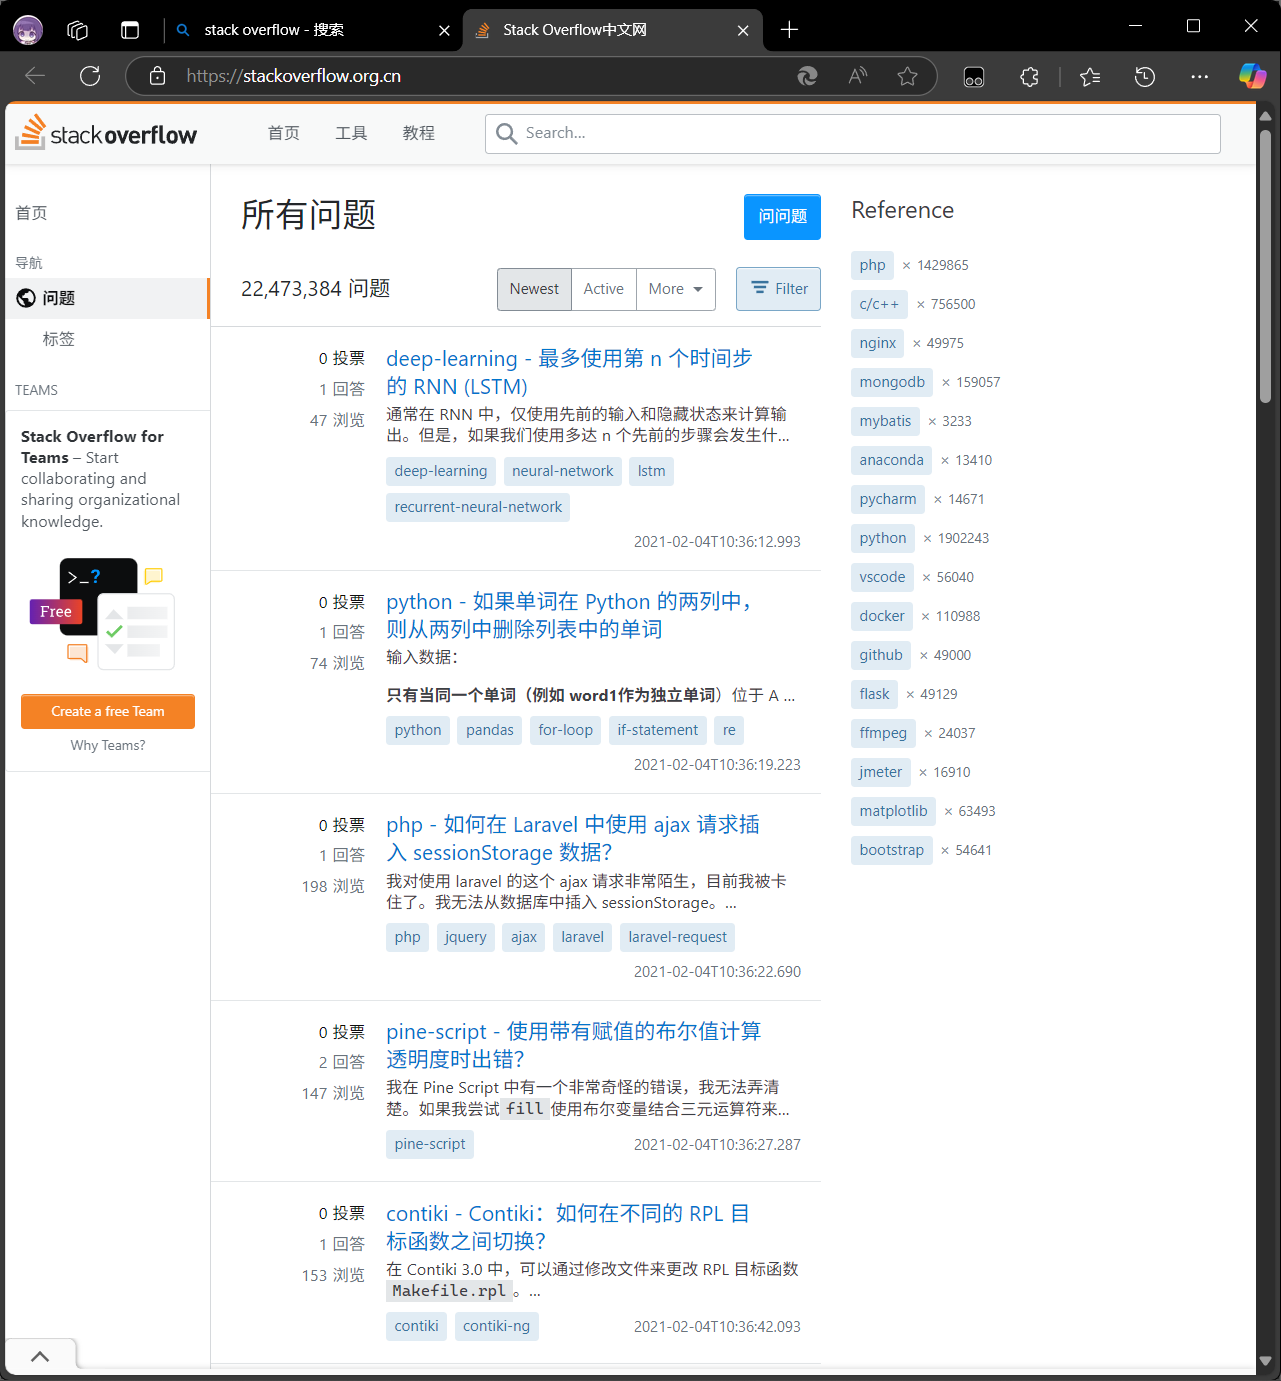
\includegraphics[width=0.9\textwidth]{4-4-StackOverflow.png}
    \end{columns}
\end{frame}

\begin{frame}{GitHub}
    \begin{columns}[T]
        \column{0.48\textwidth}
            GitHub是一个代码托管平台,用户可以在上面存储和管理自己的代码。它的内容主要是关于开源项目、代码托管和版本控制等方面的信息。我们可以在这个平台上找到很多开源项目的代码和文档,并且可以参与到这些项目中去。
        \column{0.48\textwidth}
            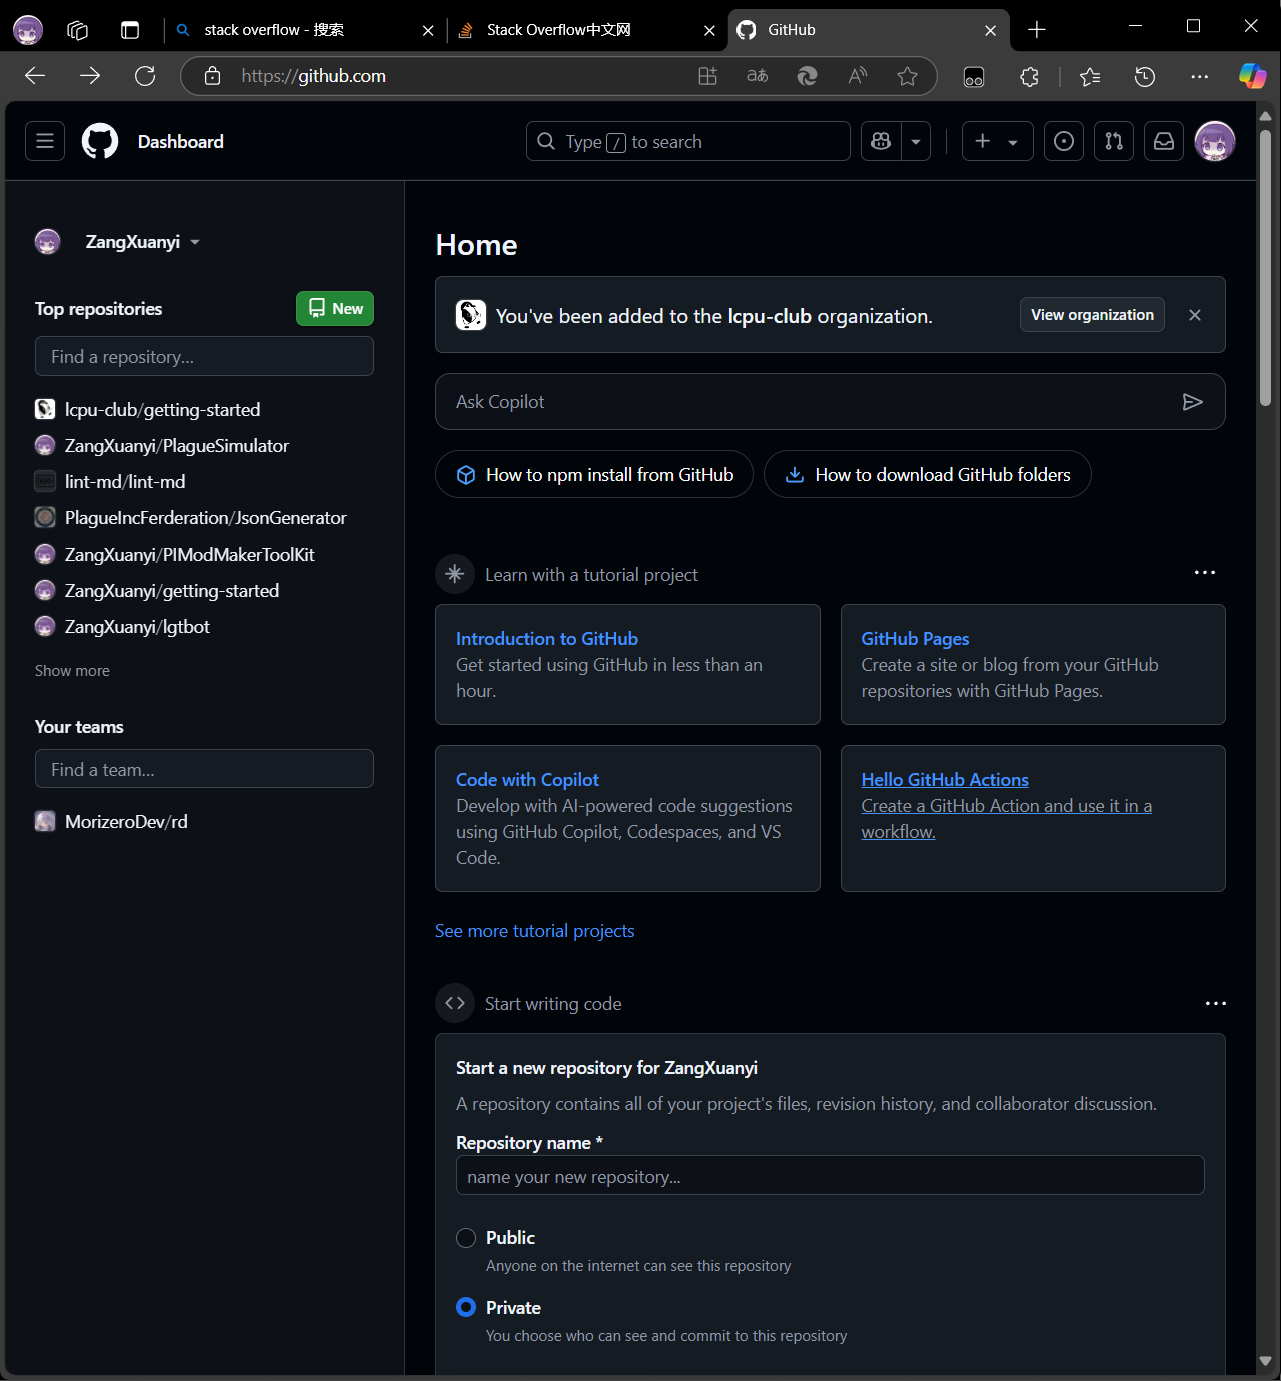
\includegraphics[width=0.9\textwidth]{4-5-GitHub.png}
    \end{columns}
\end{frame}

\begin{frame}{Wikipedia}
    维基百科是一个自由的百科全书,用户可以在上面查找和编辑各种信息。它的内容主要是关于历史、文化、科学等方面的信息。维基百科是一个非常好的信息来源,但是我们需要注意的是,它的内容并不是完全可靠的,有些信息可能是错误的或者不准确的。同时,国内有可能会无法访问该网站,这时我们可以使用一些镜像网站来访问。
    \begin{block}{小提示}<2->
        如果你在维基百科上看到了一些不准确的信息,可以通过点击页面上的“编辑”按钮来修改它。维基百科是一个开放的平台,任何人都可以参与到它的编辑中去。
    \end{block}
\end{frame}

\begin{frame}{其他著名博客和教程}
    除了上述网站,还有很多其他著名的博客和教程,例如:
    \begin{itemize}
        \item <2->W3Schools及其类似网站(菜鸟教程、W3School等)
        \item <3->OI Wiki、CTF Wiki、HPC Wiki等
        \item <4->CS自学指南
    \end{itemize}
\end{frame}

\begin{frame}{其他国内优质平台}
    \begin{columns}[T]
        \column{0.48\textwidth}
            我们一般认为国内的优质平台有:
            \begin{itemize}
                \item 知乎
                \item 博客园
                \item 简书
                \item SegmentFault
                \item Bilibili
            \end{itemize}
        \column{0.48\textwidth}
            \begin{alertblock}{特别说明}<2->
                CSDN 上虽然也有不少信息,但是该平台质量较低,商业化程度较高。虽然在少数情况下我们最终能够找到一些有用的信息,但是\textbf{高质量的平台能节约鉴别信息的精力}。
            \end{alertblock}
    \end{columns}    
\end{frame}

\subsection{语言大模型}
\begin{frame}{LLM的使用原则}
    与搜索不同,LLM的使用应该遵循以下原则:
    \begin{itemize}
        \item <2->使用自然语言而关键词;
        \item <3->使用简洁明了、没有歧义的语言;
        \item <4->使用具体的例子规范输出;
        \item <5->把困难的任务“分治”成简单的任务;
        \item <6->使用更先进的Prompt来引导模型。
    \end{itemize}
    \begin{block}{小提示}<7->
        “怎样更好地使用LLM”这个问题其实并不简单,以至于现在已经有了一门学科“提示词工程”专门研究这一问题。有兴趣的同学可以自行查找相关资料。
    \end{block}
\end{frame}

\subsection{提问的艺术}
\begin{frame}{礼貌和尊重}
    \begin{exampleblock}{例子}
        “我电脑蓝屏了,谁能来帮修一下。”
    \end{exampleblock}

    \uncover<2->{在寻求帮助时,\textbf{礼貌和尊重}是至关重要的。\textbf{没有人有义务解答你的问题},解决问题也许会耗费不少的时间和精力,大多数人解答问题往往只是出于本能的善意。礼貌的表达不仅能促使他人更愿意帮助你,还能建立良好的沟通氛围。}
\end{frame}

\begin{frame}{增加有用的信息}
    \begin{exampleblock}{例子}
        “我的电脑不知道为什么蓝屏了,我今年刚上小学二年级,那能请你帮帮我吗?谢谢,谢谢。”
    \end{exampleblock}

    \uncover<2->{即使拥有最真诚的语气,这样的问题也往往会让别人无从下手。蓝屏的可能原因有很多,而且不同的蓝屏信息也对应着可能截然不同的解决方案。如果你能够更为\textbf{具体地描述}你遇到的问题,比如蓝屏时的错误代码、蓝屏时的操作、蓝屏时的应用程序等等,那么别人就能更好地帮助你解决问题。}
\end{frame}

\begin{frame}{减少无用信息并明确化你的描述}
    \begin{exampleblock}{例子}
        “我的电脑突然蓝屏了,我今年刚上小学二年级,我的蓝屏时候遇到的代码是 XXXXXXXX,正在直面天命的时候蓝屏了。那能请你帮帮我吗?拜托了,这对我来说真的很重要!谢谢,谢谢。”
    \end{exampleblock}

    \uncover<2->{部分人在提问的时候总会无意识地强调与问题无关的东西。这种
    内容往往会显著地降低信息密度,甚至招致人的反感与厌恶。一个更常见的例子是在
    社群中发送大段语音而不是文字。同时,我们也应该避免使用一些模糊的词语,例如“突然”、“不知道为什么”等等。}
\end{frame}

\begin{frame}{列出你失败的尝试}
    \begin{exampleblock}{例子}
        “我的电脑突然蓝屏了,我的蓝屏时候遇到的代码是XXXXXXXX,是在游玩《黑
        神话·悟空》的时候突然蓝屏的。能麻烦你帮我看看吗?拜托了,非常感谢!”
    \end{exampleblock}

    \uncover<2->{虽然上述文本和诚恳、无用信息少且描述明确,但是在实际社群中依然可能会被当作“日经贴”而收到RTFM或者STFM而回答。列出你失败的尝试非但不丢人,还能表现出你为了自己解决自己遇到的问题所付出的努力,也能够显著地减少重复劳动与受到上述回复。}
\end{frame}

\begin{frame}{一个较好的提问}
    \begin{exampleblock}{例子}
        “我的电脑突然蓝屏了,我的蓝屏时候遇到的代码是XXXXXXXX,是在游玩《黑
神话·悟空》的时候突然蓝屏的。我上网搜索了代码相关的错误信息,尝试了网上可能
有用的A 方法和B 方法,但都没有奏效。能麻烦你帮我看看吗?拜托了,非常感谢!”
    \end{exampleblock}

    一个较好的提问诞生了!
\end{frame}


\end{document}